
\documentclass[]{article}

\usepackage[utf8]{inputenc}
\usepackage{graphicx}
\usepackage{pgfplots}
\usetikzlibrary{calc,patterns,angles,quotes,arrows}
\usepackage{tikz}
\usetikzlibrary{datavisualization}
\usetikzlibrary{matrix}
\usepackage{pgfplots}

\title{Utility Functions Plots}
\author{Giacomo Vagni}
\date{May 2023}

\begin{document}

\maketitle

\begin{figure}
	\centering
	\caption{Substitute Goods}
\begin{center}
	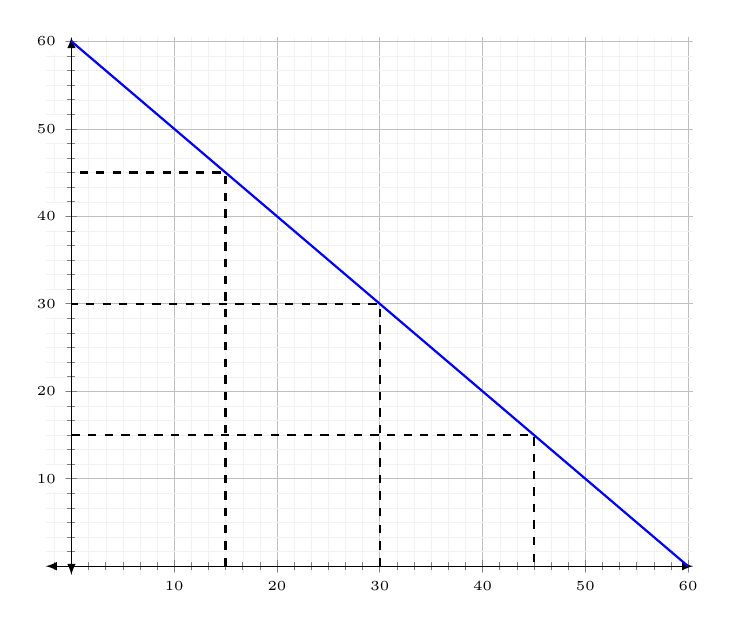
\begin{tikzpicture}
	\begin{axis}[
scale = 1.2,
xmin=-2,xmax=60,
ymin=-0.5,ymax=60,
grid=both,
grid style={line width=.1pt, draw=gray!10},
major grid style={line width=.2pt,draw=gray!50},
axis lines=middle,
minor tick num=5,
enlargelimits={abs=0.5},
axis line style={latex-latex},
ticklabel style={font=\tiny,fill=white},
xlabel style={at={(ticklabel* cs:1)},anchor=north west},
ylabel style={at={(ticklabel* cs:1)},anchor=south west}
]

	
	scale = 1.2,
	xmin = 0, xmax = 65,
	ymin = 0, ymax = 65,
	axis lines* = left,
	xtick = {15,30,45, 60}, 
	ytick = {15,30,45, 60}, 
	clip = false,
	]
	\addplot[domain = 0:60, restrict y to domain = 0:60, samples = 400, color = blue, thick]{60-1.0*x};
	% Labels
	\node [right] at (current axis.right of origin) {Tennis};
	\node [above] at (current axis.above origin) {Badminton};
	
	\addplot[color = black, dashed, thick] coordinates {(15, 0) (15, 45) (0, 45)};
	\addplot[color = black, dashed, thick] coordinates {(30, 0) (30, 30) (0, 30)};
	\addplot[color = black, dashed, thick] coordinates {(0, 15) (45, 15) (45, 0)};
	
	\end{axis}
	\end{tikzpicture}
\end{center}
\end{figure}



\begin{figure}
	\centering
	\caption{Diminishing Marginal Utility}
\begin{center}
	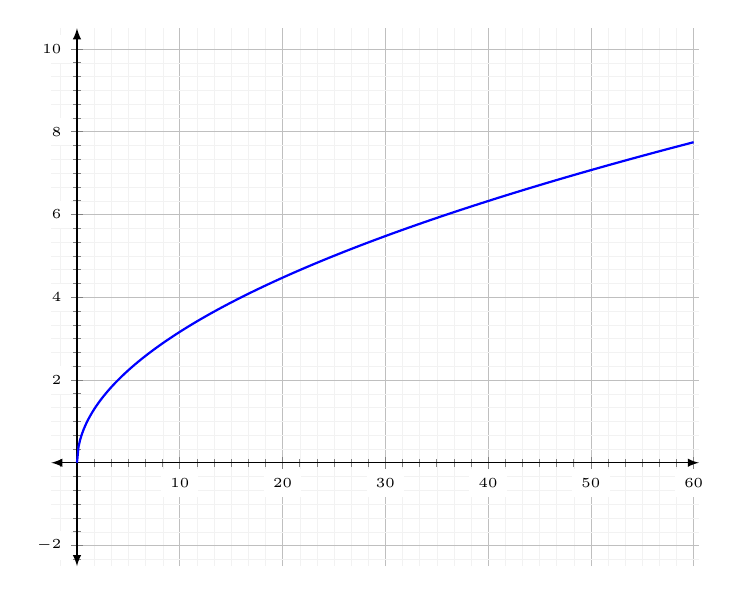
\begin{tikzpicture}
	\begin{axis}[
scale = 1.2,
xmin=-2,xmax=60,
ymin=-2,ymax=10,
grid=both,
grid style={line width=.1pt, draw=gray!10},
major grid style={line width=.2pt,draw=gray!50},
axis lines=middle,
minor tick num=5,
enlargelimits={abs=0.5},
axis line style={latex-latex},
ticklabel style={font=\tiny,fill=white},
xlabel style={at={(ticklabel* cs:1)},anchor=north west},
ylabel style={at={(ticklabel* cs:1)},anchor=south west}
]
	
	\addplot[domain = 0:60, restrict y to domain = 0:15, samples = 400, color = blue, thick]{x^0.5};
	% Labels
	\node [right] at (current axis.right of origin) {$x1$};
	\node [above] at (current axis.above origin) {Happiness};
	
	%\addplot[color = black, dashed, thick] coordinates {(30, 0) (30, 5.5) (0, 5.5)};
	%\addplot[domain = 0:60, restrict y to domain = 0:60, samples = 400, color = red]{ 900/x };
	
	\end{axis}
	\end{tikzpicture}
\end{center}
\end{figure}


\begin{figure}
	\centering
	\caption{Indifference Curve}
\begin{center}
	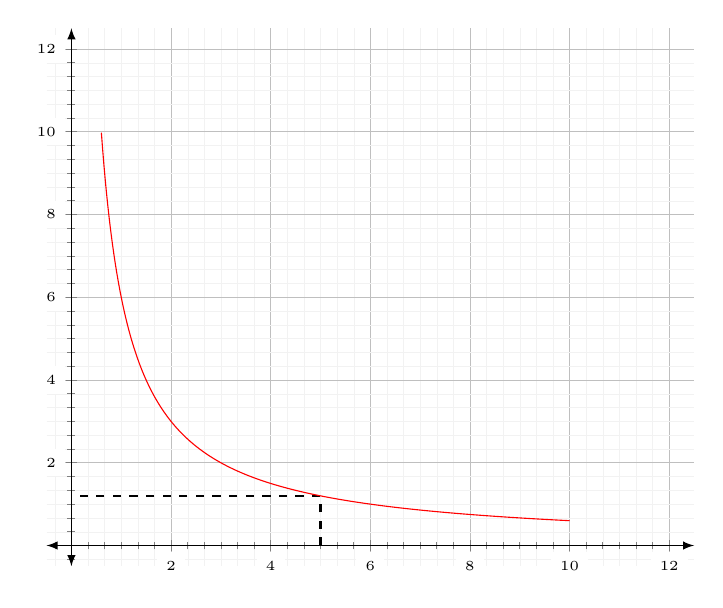
\begin{tikzpicture}
	\begin{axis}[
scale = 1.2,
xmin=0,xmax=12,
ymin=0,ymax=12,
grid=both,
grid style={line width=.1pt, draw=gray!10},
major grid style={line width=.2pt,draw=gray!50},
axis lines=middle,
minor tick num=5,
enlargelimits={abs=0.5},
axis line style={latex-latex},
ticklabel style={font=\tiny,fill=white},
xlabel style={at={(ticklabel* cs:1)},anchor=north west},
ylabel style={at={(ticklabel* cs:1)},anchor=south west}
]

	\node [right] at (current axis.right of origin) {$x1$};
	\node [above] at (current axis.above origin) {$x2$};

	\node [above, color = red] at (100,10) {U = 6};
		
	\addplot[color = black, dashed, thick] coordinates {(5, 0) (5, 1.2) (0, 1.2)};
	
	\addplot[domain = 0:10, restrict y to domain = 0:10, samples = 400, color = red]{ 6/x };
	
	\end{axis}
	\end{tikzpicture}
\end{center}
\end{figure}


\begin{figure}
	\centering
	\caption{Indifference Curve for Utility of 5 vs Utility of 3}
\begin{center}
	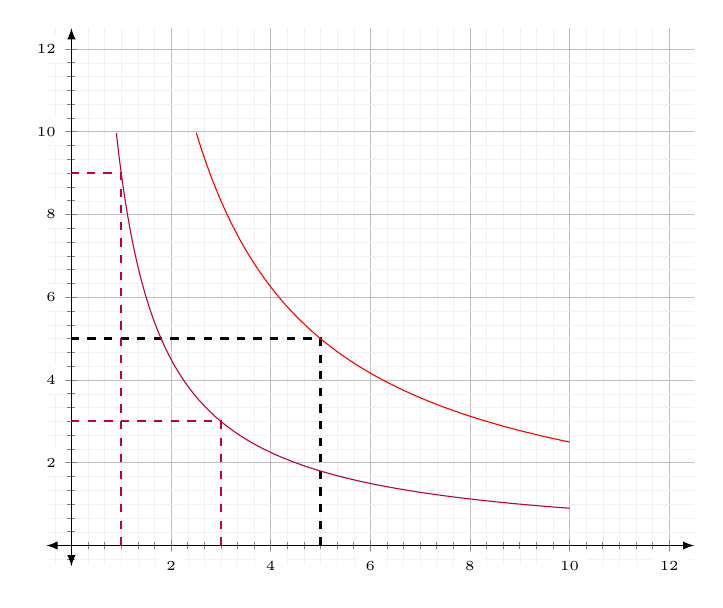
\begin{tikzpicture}
	\begin{axis}[
scale = 1.2,
xmin=0,xmax=12,
ymin=0,ymax=12,
grid=both,
grid style={line width=.1pt, draw=gray!10},
major grid style={line width=.2pt,draw=gray!50},
axis lines=middle,
minor tick num=5,
enlargelimits={abs=0.5},
axis line style={latex-latex},
ticklabel style={font=\tiny,fill=white},
xlabel style={at={(ticklabel* cs:1)},anchor=north west},
ylabel style={at={(ticklabel* cs:1)},anchor=south west}
]

	\node [right] at (current axis.right of origin) {$x1$};
	\node [above] at (current axis.above origin) {$x2$};
	
	\node [above, color = red] at (100,30) {U = 5};
	
	\addplot[color = black, dashed, thick] coordinates {(5, 0) (5, 5) (0, 5)};
	
	\addplot[domain = 0:10, restrict y to domain = 0:10, samples = 400, color = red]{ (5/(x^0.5))^(1/0.5) };
	
		\node [above, color = purple] at (100,10) {U = 3};
		
	\addplot[domain = 0:10, restrict y to domain = 0:10, samples = 400, color = purple]{ (3/(x^0.5))^(1/0.5) };
	
	\addplot[color = purple, dashed, thick] coordinates {(1, 0) (1, 9) (0, 9)};
	\addplot[color = purple, dashed, thick] coordinates {(3, 0) (3, 3) (0, 3)};
			
	\end{axis}
	\end{tikzpicture}
\end{center}
\end{figure}


\begin{figure}
	\centering
	\caption{Budget Line}
\begin{center}
	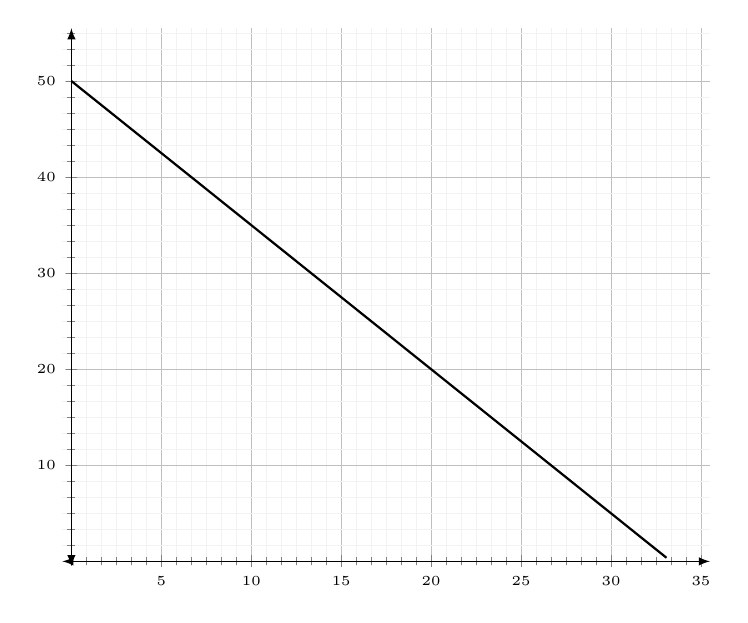
\begin{tikzpicture}
\begin{axis}[
scale = 1.2,
xmin=0,xmax=35,
ymin=0,ymax=55,
grid=both,
grid style={line width=.1pt, draw=gray!10},
major grid style={line width=.2pt,draw=gray!50},
axis lines=middle,
minor tick num=5,
enlargelimits={abs=0.5},
axis line style={latex-latex},
ticklabel style={font=\tiny,fill=white},
xlabel style={at={(ticklabel* cs:1)},anchor=north west},
ylabel style={at={(ticklabel* cs:1)},anchor=south west}
]

	\addplot[domain = 0:100, restrict y to domain = 0:100, samples = 400, color = black, thick]{(50-1.5*x)};
	% Labels
	\node [right] at (current axis.right of origin) {$x$};
	\node [above] at (current axis.above origin) {$y$};
	
	\end{axis}
	\end{tikzpicture}
\end{center}
\end{figure}


\begin{figure}
	\centering
	\caption{Optimal Bundle}
\begin{center}
	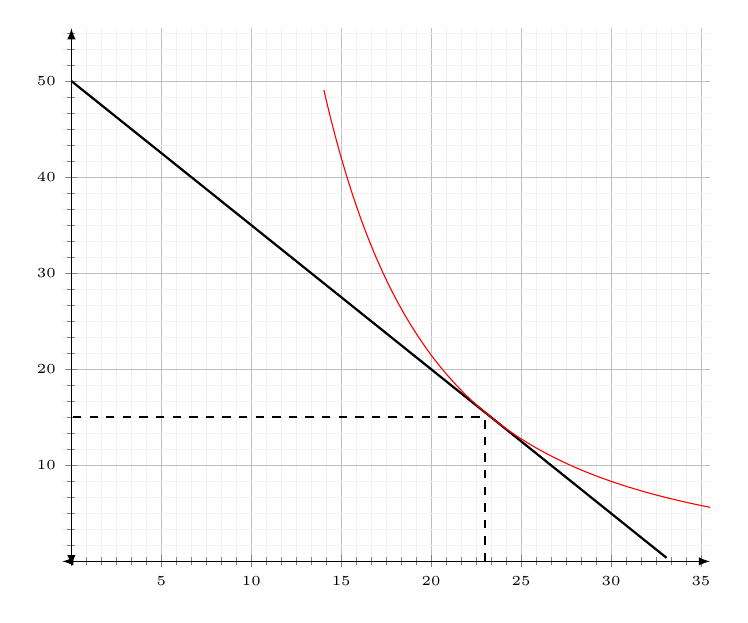
\begin{tikzpicture}
	\begin{axis}[
	scale = 1.2,
	xmin=0,xmax=35,
	ymin=0,ymax=55,
	grid=both,
	grid style={line width=.1pt, draw=gray!10},
	major grid style={line width=.2pt,draw=gray!50},
	axis lines=middle,
	minor tick num=5,
	enlargelimits={abs=0.5},
	axis line style={latex-latex},
	ticklabel style={font=\tiny,fill=white},
	xlabel style={at={(ticklabel* cs:1)},anchor=north west},
	ylabel style={at={(ticklabel* cs:1)},anchor=south west}
	]
	
	\addplot[domain = 0:100, restrict y to domain = 0:100, samples = 400, color = black, thick]{(50-1.5*x)};
	% Labels
	\node [right] at (current axis.right of origin) {$x$};
	\node [above] at (current axis.above origin) {$y$};
	
	\addplot[color = black, dashed, thick] coordinates {(23, 0) (23, 15) (0, 15)};	
		
	\addplot[domain = 0:50, restrict y to domain = 0:50, samples = 400, color = red]{ (20.43191/x^0.7)^(1/0.3) };
			
	\end{axis}
	\end{tikzpicture}
\end{center}
\end{figure}

\end{document}
